\documentclass[12pt]{article}
\usepackage[margin=1in]{geometry}
\usepackage{listings}
\usepackage{graphicx}
\usepackage{float}
\usepackage{color} %red, green, blue, yellow, cyan, magenta, black, white
\definecolor{mygreen}{RGB}{28,172,0} % color values Red, Green, Blue
\definecolor{mylilas}{RGB}{170,55,241}

\setlength{\parskip}{1em}

\lstset{language=Matlab,%
    %basicstyle=\color{red},
    breaklines=true,%
    morekeywords={matlab2tikz},
    keywordstyle=\color{blue},%
    morekeywords=[2]{1}, keywordstyle=[2]{\color{black}},
    identifierstyle=\color{black},%
    stringstyle=\color{mylilas},
    commentstyle=\color{mygreen},%
    showstringspaces=false,%without this there will be a symbol in the places where there is a space
    numbers=left,%
    numberstyle={\tiny \color{black}},% size of the numbers
    numbersep=9pt, % this defines how far the numbers are from the text
    emph=[1]{for,end,break},emphstyle=[1]\color{red}, %some words to emphasise
    %emph=[2]{word1,word2}, emphstyle=[2]{style},    
}

\usepackage{mathtools}
\usepackage{url}

\title{Assignment 3, COMP4702}
\author{Roy Portas, 43560846}
\date{\today}

\begin{document} 
\begin{titlepage}
    \maketitle
\end{titlepage}

\section*{Prac 7}

\subsection*{Q 7.1}

\subsubsection*{Part A}

The network topology that was used is Prac 6 is a 60 unit neural network with one hidden layer.
Five different methods were compared, with learning rates ranging from 0.001 to 10.
For this test 100 was chosen as the maximum steps, 
this is relatively small but increasing the maximum steps should only make the model more accurate.

\begin{figure}[H]
	\centering
	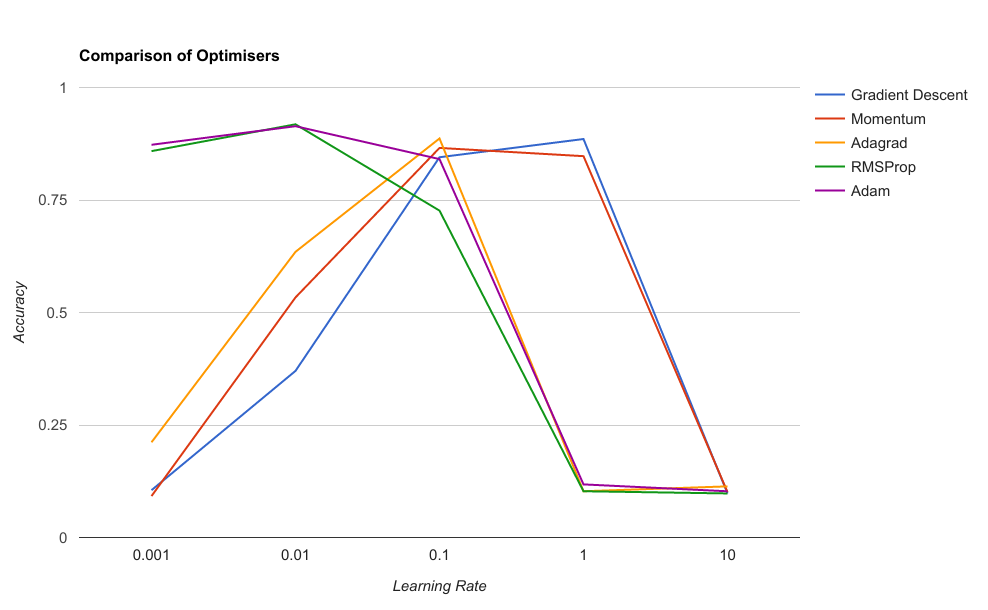
\includegraphics[width=\linewidth]{images/q7_optimisers}
\end{figure}

The above figure shows a comparison of different methods with different learning rates.
It can be seen that RMSProp and Adam run much better with smaller learning rates, with Adam slightly outperforming RMSProp.

Gradient Descent and Momentum work better with higher learning rates, peaking with a learning rate of 1, with Gradient Descent performing the best of the two.

Adagrad performs the best with a learning rate of 0.1, however does not perform well with higher or lower values, whereas all the other methods work well for multiple learning rates.

All the algorithms start performing poorly when the learning rate increases past 1. The best performing algorithm was RMSProp with a learning rate of 0.01, with an accuracy of 0.9182.

\subsubsection*{Part B}

The Adam method was chosen for question with a learning rate of 0.01, beta1 of 0.9 and beta2 of 0.8.
The choices for the activation functions are Relu, Tanh and Sigmoid, which are shown in the figure below.

\begin{figure}[H]%
    \centering
    \subfloat[Relu]{{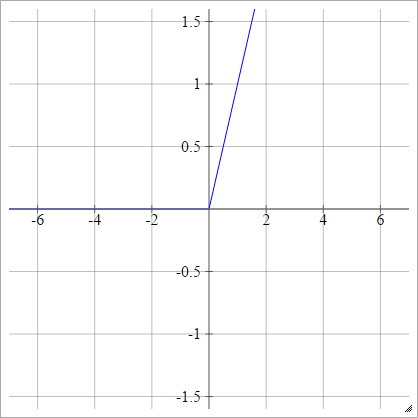
\includegraphics[width=0.2\linewidth]{images/activation_functions/relu} }}%
    \qquad
    \subfloat[Tanh]{{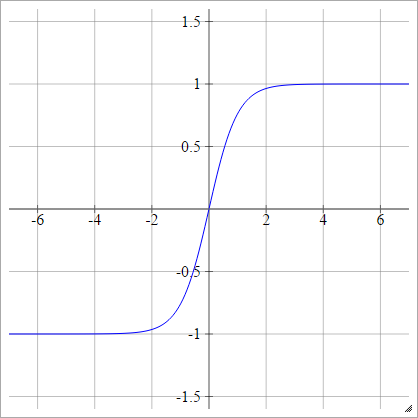
\includegraphics[width=0.2\linewidth]{images/activation_functions/tanh} }}%
    \qquad
    \subfloat[Sigmoid]{{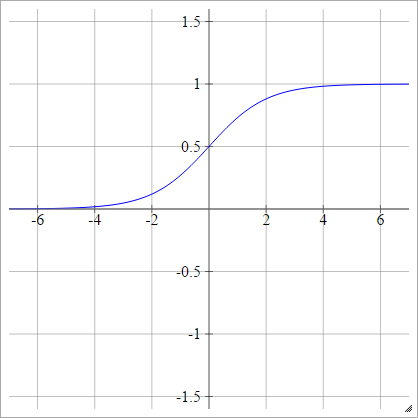
\includegraphics[width=0.2\linewidth]{images/activation_functions/sigmoid} }}%
    \caption{Activation Functions, source: \protect\url{http://cs231n.github.io/neural-networks-1}}%
\end{figure}

A few things can be attained from the above diagrams.
The Relu function has a y range from 0 to infinity, whereas tanh is bounded between -1 and 1, and sigmoid is bounded between 0 and 1.
This means that Relu won't be affected by the vanishing gradient problem, this is because the y range for Relu goes to Infinity, whereas the others converge. Having a non infinite range is better for gradient based methods, as it tends to be more stable.

\begin{figure}[H]%
    \centering
    \subfloat[Relu]{{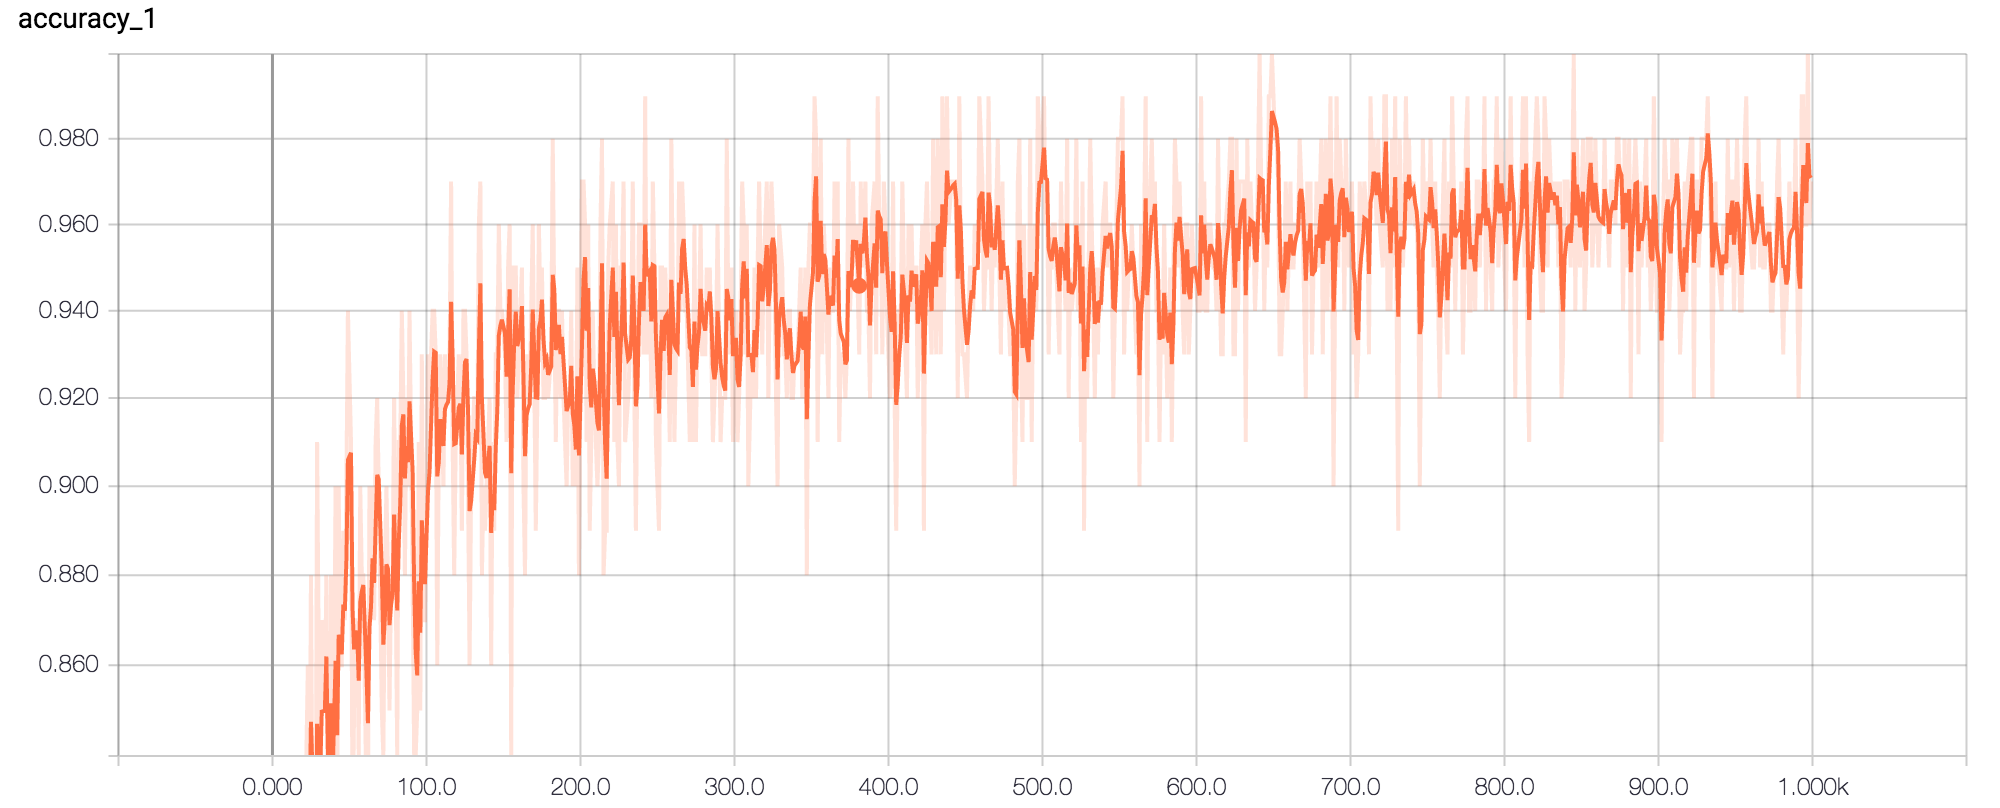
\includegraphics[width=0.7\linewidth]{images/q7_testing_relu_accuracy} }}%
    \qquad
    \subfloat[Tanh]{{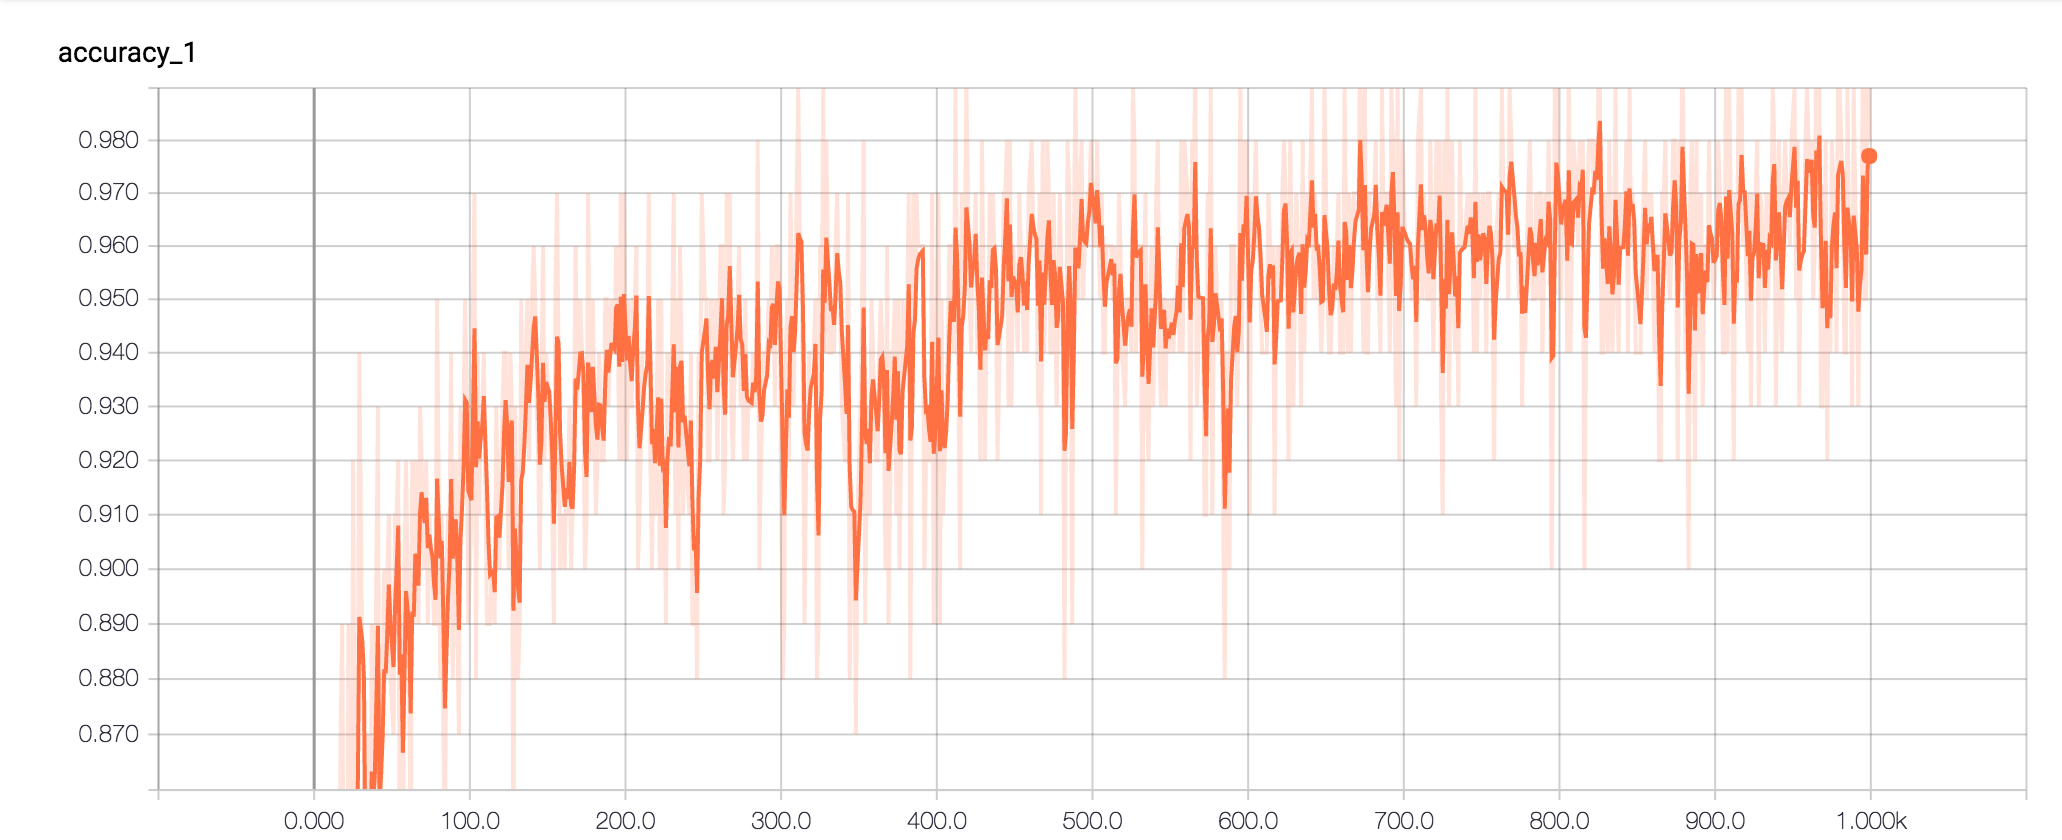
\includegraphics[width=0.7\linewidth]{images/q7_testing_tanh_accuracy} }}%
    \qquad
    \subfloat[Sigmoid]{{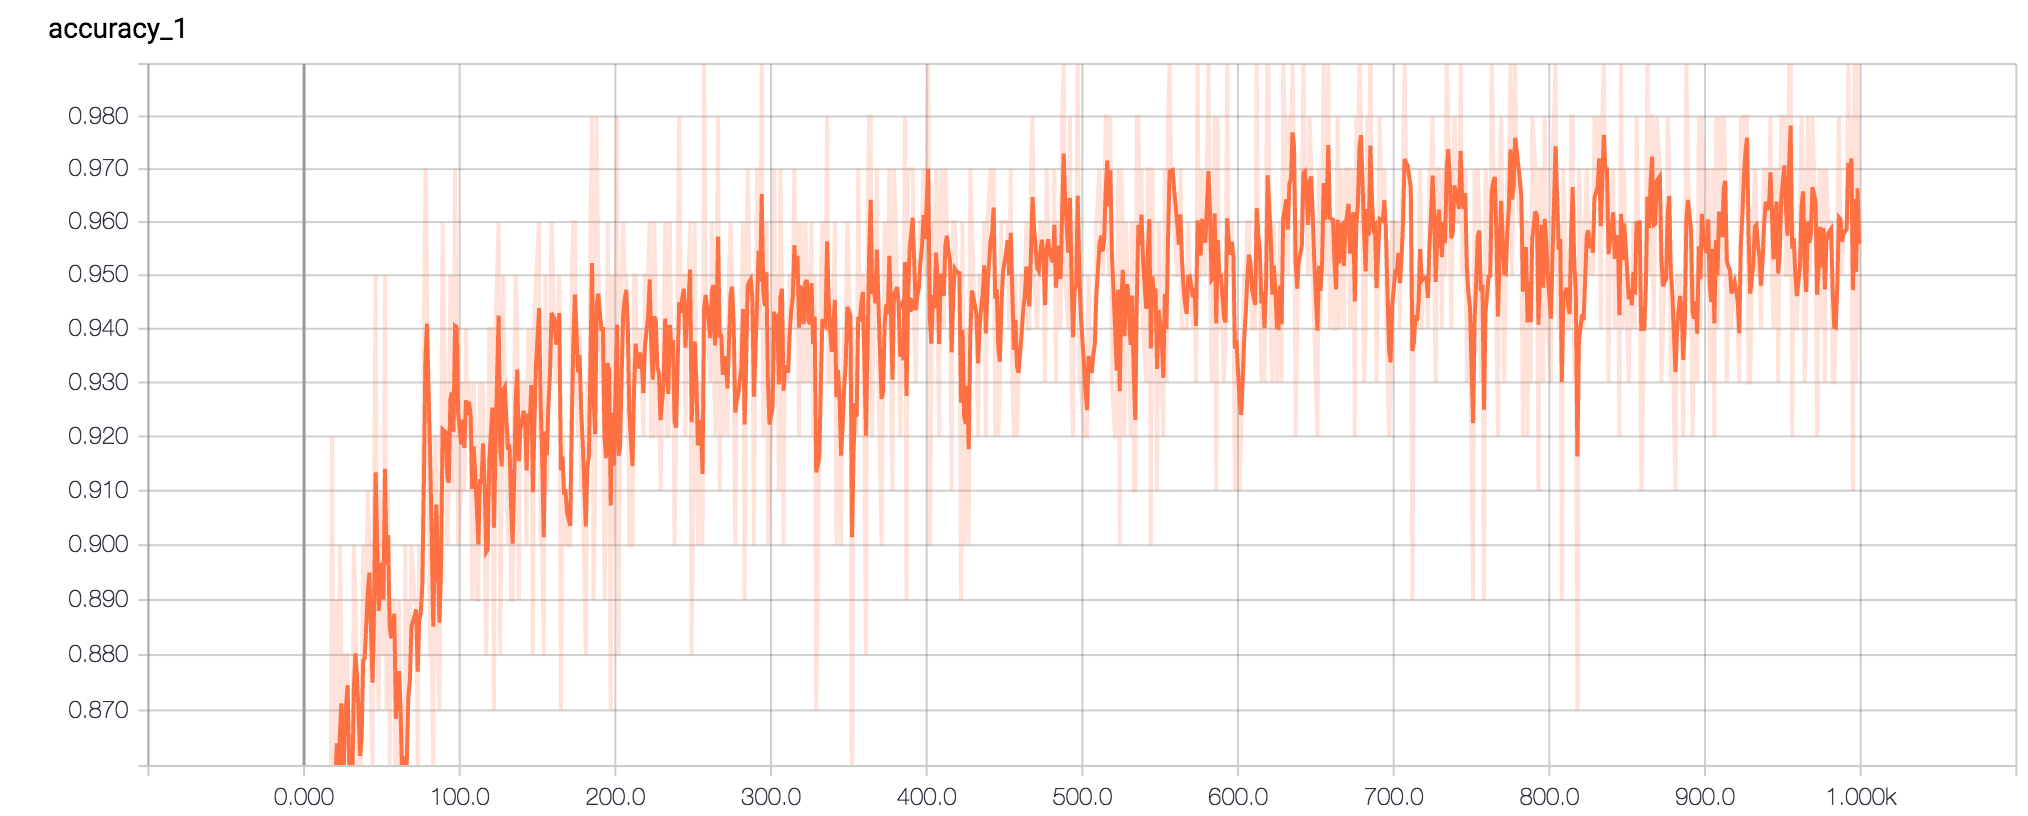
\includegraphics[width=0.7\linewidth]{images/q7_testing_sigmoid_accuracy} }}%
    \caption{Activation Function Accuracy}%
\end{figure}

From comparing the three graphs of accuracy, it can be seen that Relu seems to be the most stable, whereas both Tanh and Sigmoid has a lot more variation.

\begin{figure}[H]%
    \centering
    \subfloat[Relu]{{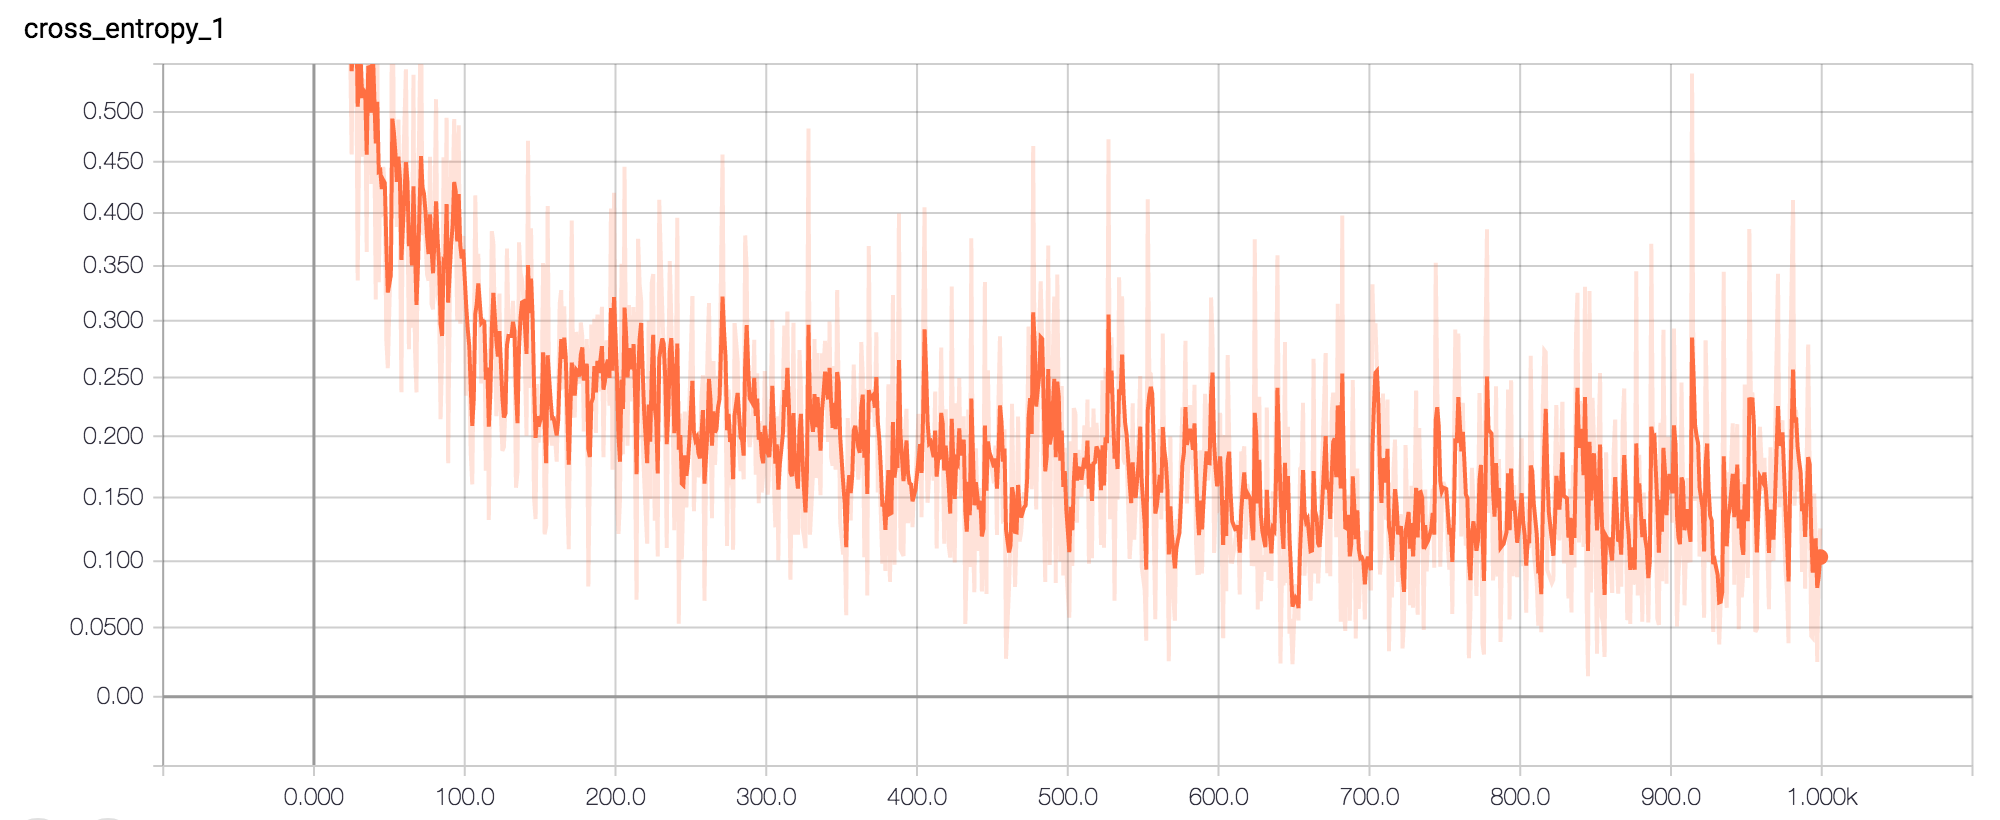
\includegraphics[width=0.7\linewidth]{images/q7_testing_relu_cross_entropy} }}%
    \qquad
    \subfloat[Tanh]{{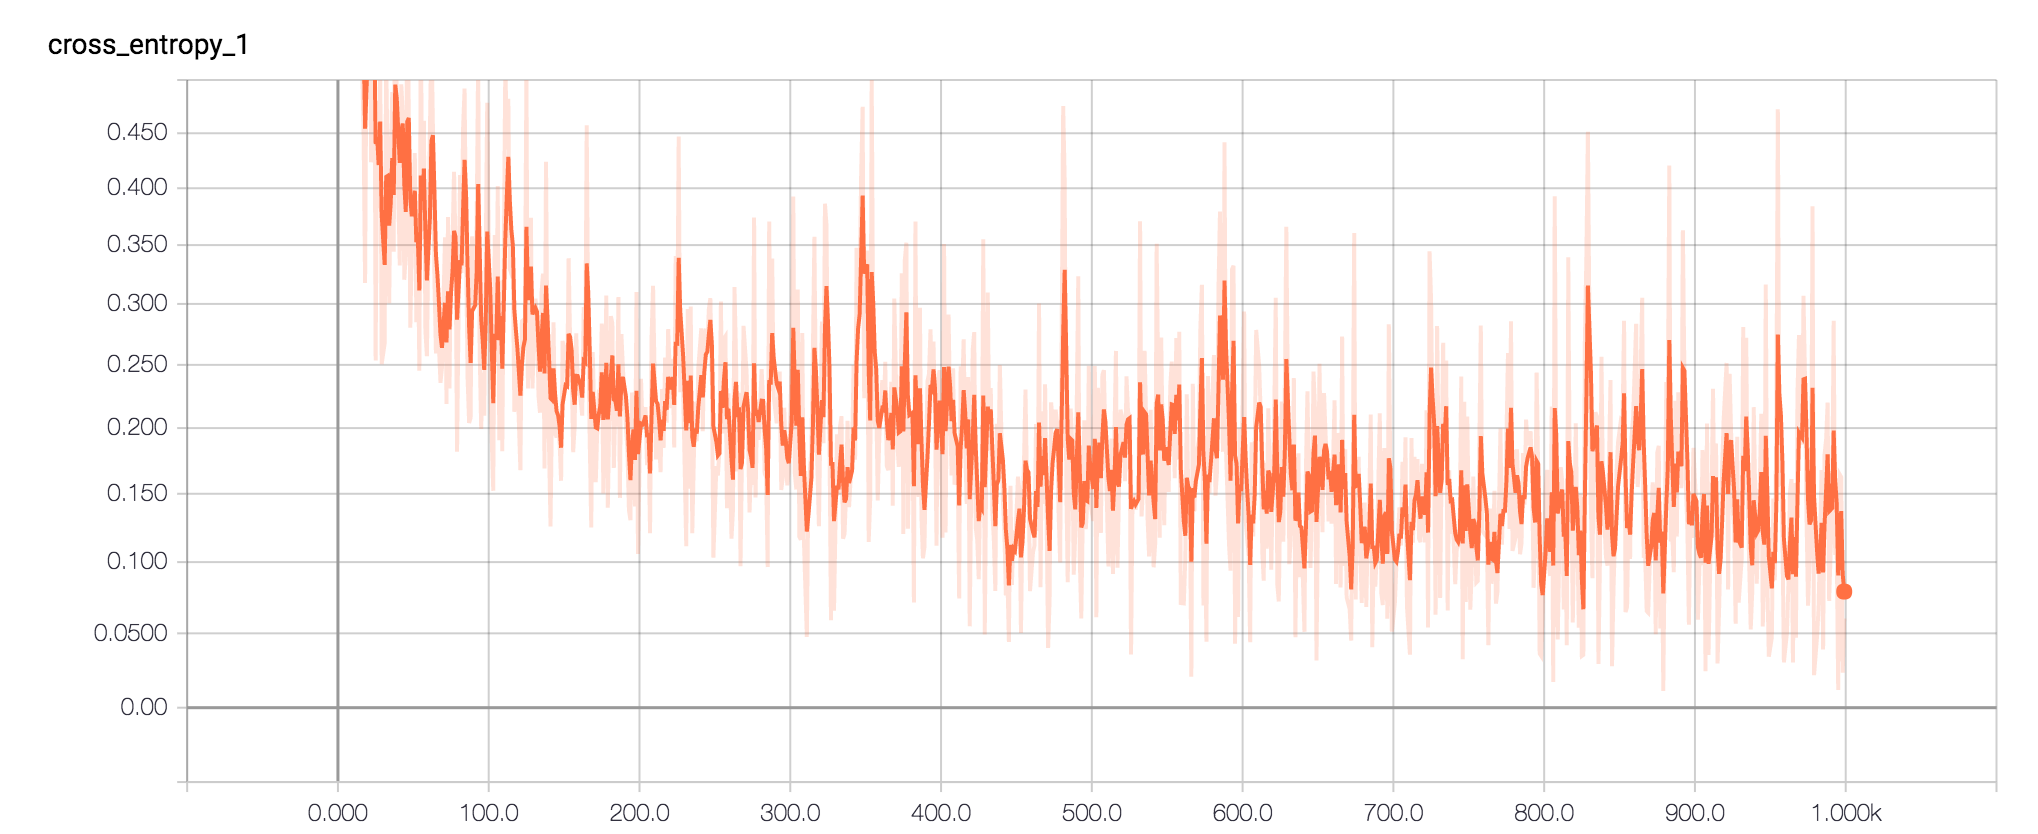
\includegraphics[width=0.7\linewidth]{images/q7_testing_tanh_cross_entropy} }}%
    \qquad
    \subfloat[Sigmoid]{{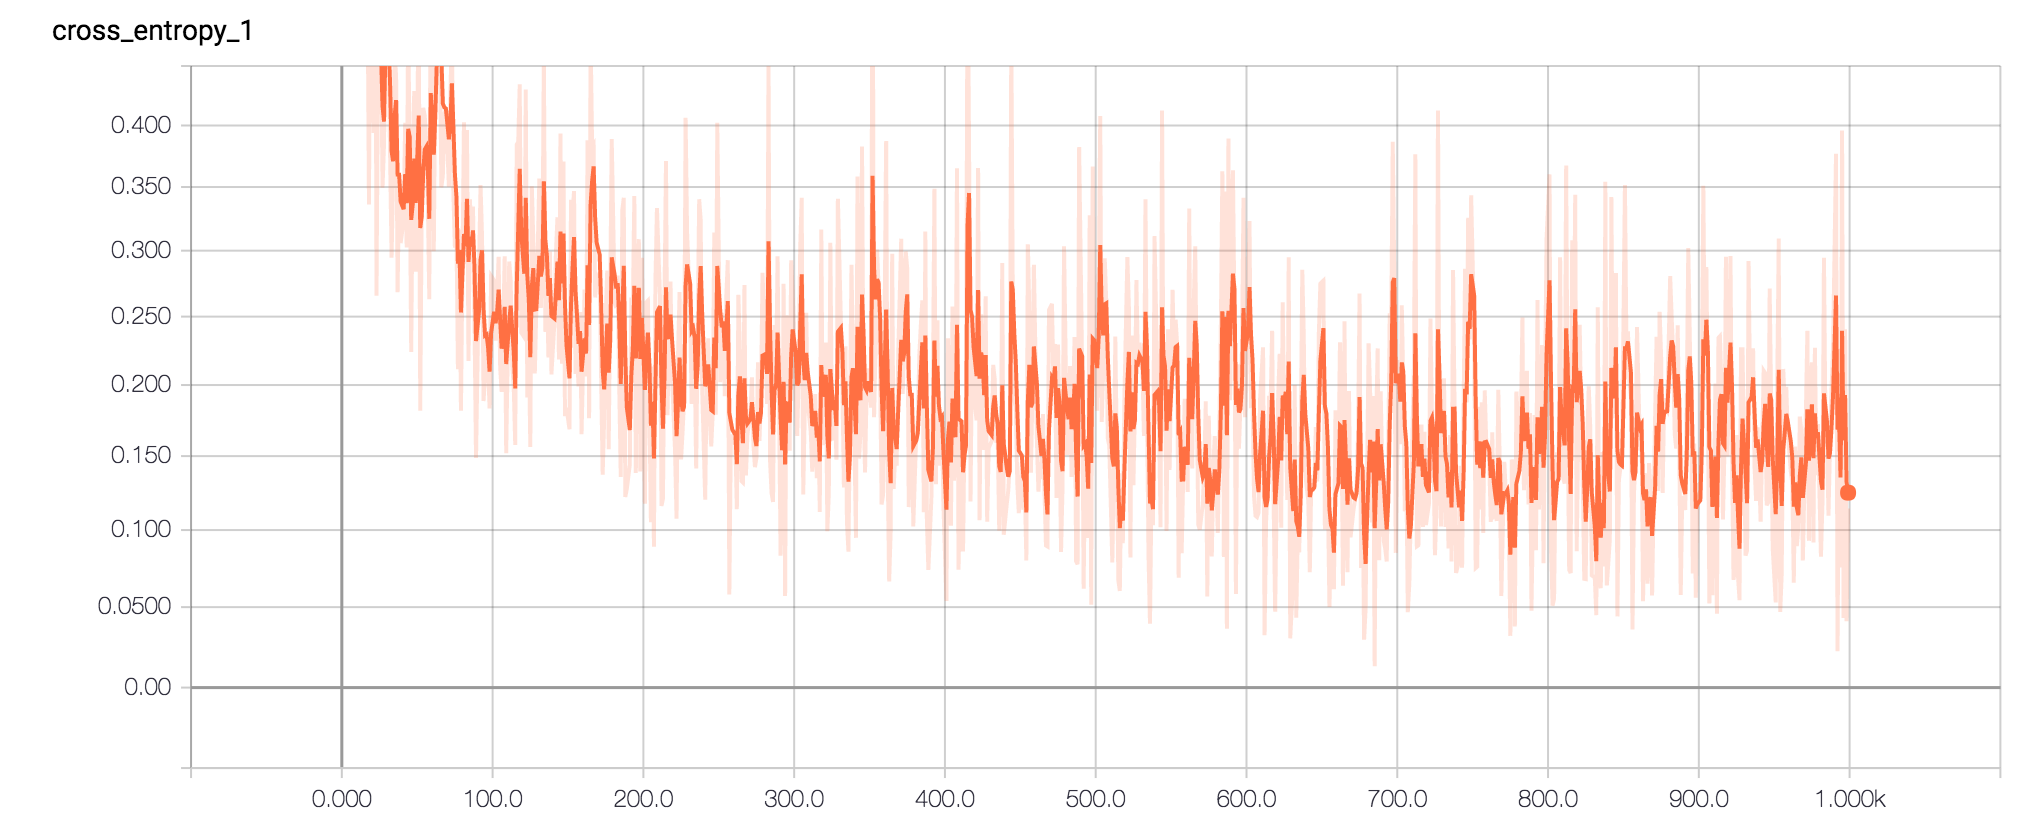
\includegraphics[width=0.7\linewidth]{images/q7_testing_sigmoid_cross_entropy} }}%
    \caption{Activation Function Cross Entropy}%
\end{figure}

The cross entropy graphs show the same relationship, with Relu having the least variation per step.

The Adam method with 1000 steps was tested using each activation function, which produced the following graph.

\begin{figure}[H]
	\centering
	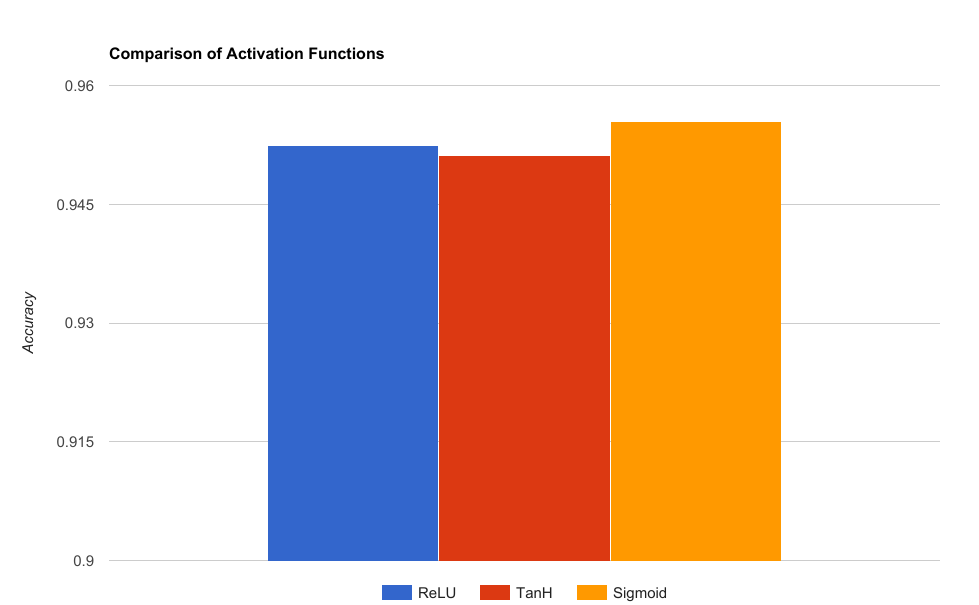
\includegraphics[width=\linewidth]{images/q7_activation_comparison}
\end{figure}

From the above graph it can be seen that changing the activation function does not make a significant difference to the accuracy, but the sigmoid function had the best accuracy from the three.

\subsection*{Q 7.2}

\subsubsection*{Volume of Weight Matrices}

The given convolutional network has two conv-pool layers followed by two fully connected layers.
The MNIST dataset is being used, so the input data will be greyscale images of size 28 pixels squared,
which can be represented as $\big[ 28 \times 28 \times 1 \big]$

The first conv layer will have 32 filters, so have a size of $\big [28 \times 28 \times 32 \big]$.
This is followed by a Relu operation but the layer size will remain the same.

The pool layer will decrease the size of the layer as it is using downsampling, this can be calculated using the following formula,
where $W$ is the input volume size, $F$ is the spacial extent and $S$ is the stride.

\begin{align*}
	size &= \frac{W - F}{S} + 1 \\
	&= \frac{28 - 2}{1} + 1\\
	&= 27
\end{align*}

Thus the size of the first pool layer is $\big[ 27 \times 27 \times 32 \big]$.

The second conv layer will have 64 filters, so a size of $\big [27 \times 27 \times 64 \big]$.

Using the equation from before the second pool layer will have a size of $\big [26 \times 26 \times 64 \big]$.

The first fully connected layer will have a size of $\big [1 \times 1 \times 1024 \big]$.

The second fully connected layer will have a size of $\big [1 \times 1 \times 10 \big]$.

\subsubsection*{Number of Parameters}

Equation for input layer:

The input layer has no bias or weights
\begin{align*}
	params &= 0
\end{align*}

Equation for calculating the parameters of the first conv layer:

\begin{align*}
	params &= unique\ weights \times filter\ size \times filter\ size \times input\ depth + bias \\
	&= 32 \times 3 \times 3 \times 1 + 32\\
	&= 320
\end{align*}

Equation for first pooling layer:

The pooling layers have no bias or weights
\begin{align*}
	params &= 0
\end{align*}

Equation for calculating the parameters of the second conv layer:

\begin{align*}
	params &= unique\ weights \times filter\ size \times filter\ size \times input\ depth + bias\\
	&= 64 \times 3 \times 3 \times 32 + 64\\
	&= 18,496
\end{align*}

Equation for second pooling layer:

The pooling layers have no bias or weights
\begin{align*}
	params &= 0
\end{align*}

Equation for the first fully connected layer:

\begin{align*}
	params &= input\ height \times input\ width \times input\ depth \times depth + bias\\
	&= 26 \times 26 \times 64 \times 1024 + 1024\\
	&= 44,303,360
\end{align*}

Equation for the second fully connected layer:

\begin{align*}
	params &= input\ height \times input\ width \times input\ depth \times depth + bias\\
	&= 1 \times 1 \times 1024 \times 10 + 10\\
	&= 10,250
\end{align*}

The total number of parameters is the sum of all the individual parameters

\begin{align*}
	total &= \sum params\\
	&= 0 + 320 + 0 + 18,496 + 0 + 44,303,360 + 10,250\\
	&= 44,332,426
\end{align*}

\subsection*{Q 7.4}


The CNN network was compared against an MLP with the same activation and optimisation function.
In this case RMSProp was chosen with a learning parameter of 0.01 and Relu was used as the activation function.

The network was tested with step sizes of 100, 300, 600, 1000 and 2000.

\begin{table}
\centering
\begin{tabular}{|c|c|c|}
\hline
Steps & MLP & CNN \\
\hline
100 & 0.90140003 & 0.95289999 \\
300 & 0.90689999 & 0.97460002 \\
600 & 0.95490003 & 0.977 \\
1000 & 0.95230001 & 0.97970003 \\
2000 & 0.96619999 & 0.98259997 \\
\hline
\end{tabular}
\end{table}

\begin{figure}[H]
	\centering
	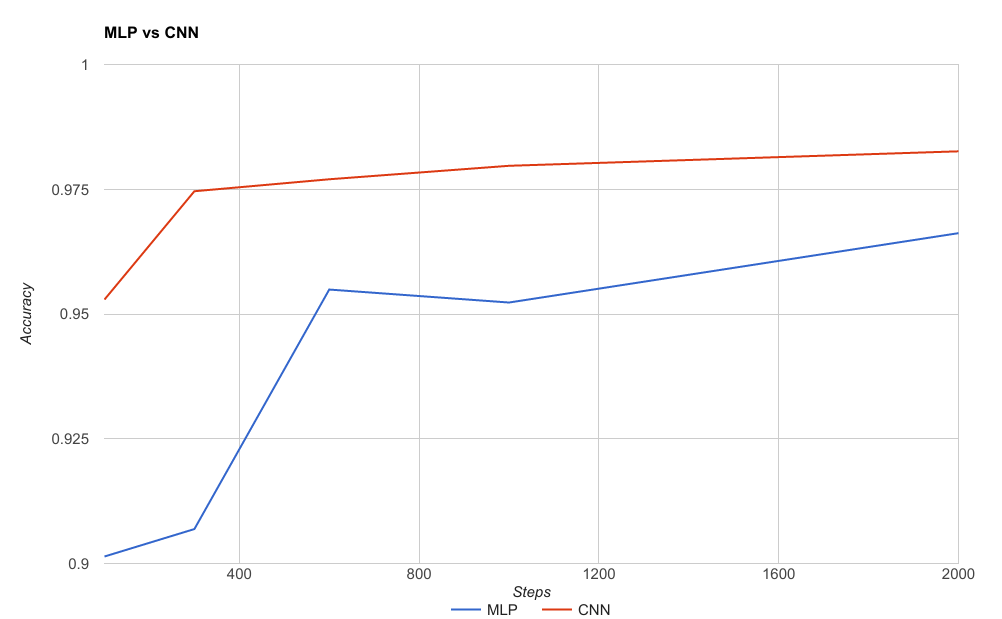
\includegraphics[width=\linewidth]{images/q7_cnn_vs_mlp}
\end{figure}

From the chart it can be seen that the CNN has the best performance regardless of step size,
performing significantly better than MLP when tested with 100 steps.
When the step size is increased the performance becomes closer,
thus in theory the MLP can reach similar performance with a very large step size.

Its also worth nothing that the CNN network took far longer to train than the MLP.

\section*{Prac 8}

\subsection*{Q 8.3}

The best result from the Q2 was found to be a polynomial kernel function with epsilon parameter of 1.
This kernel was used with varying parameters for C, which produced the following graph

\begin{figure}[H]
	\centering
	\caption{Performance vs Perplexity Parameter}
	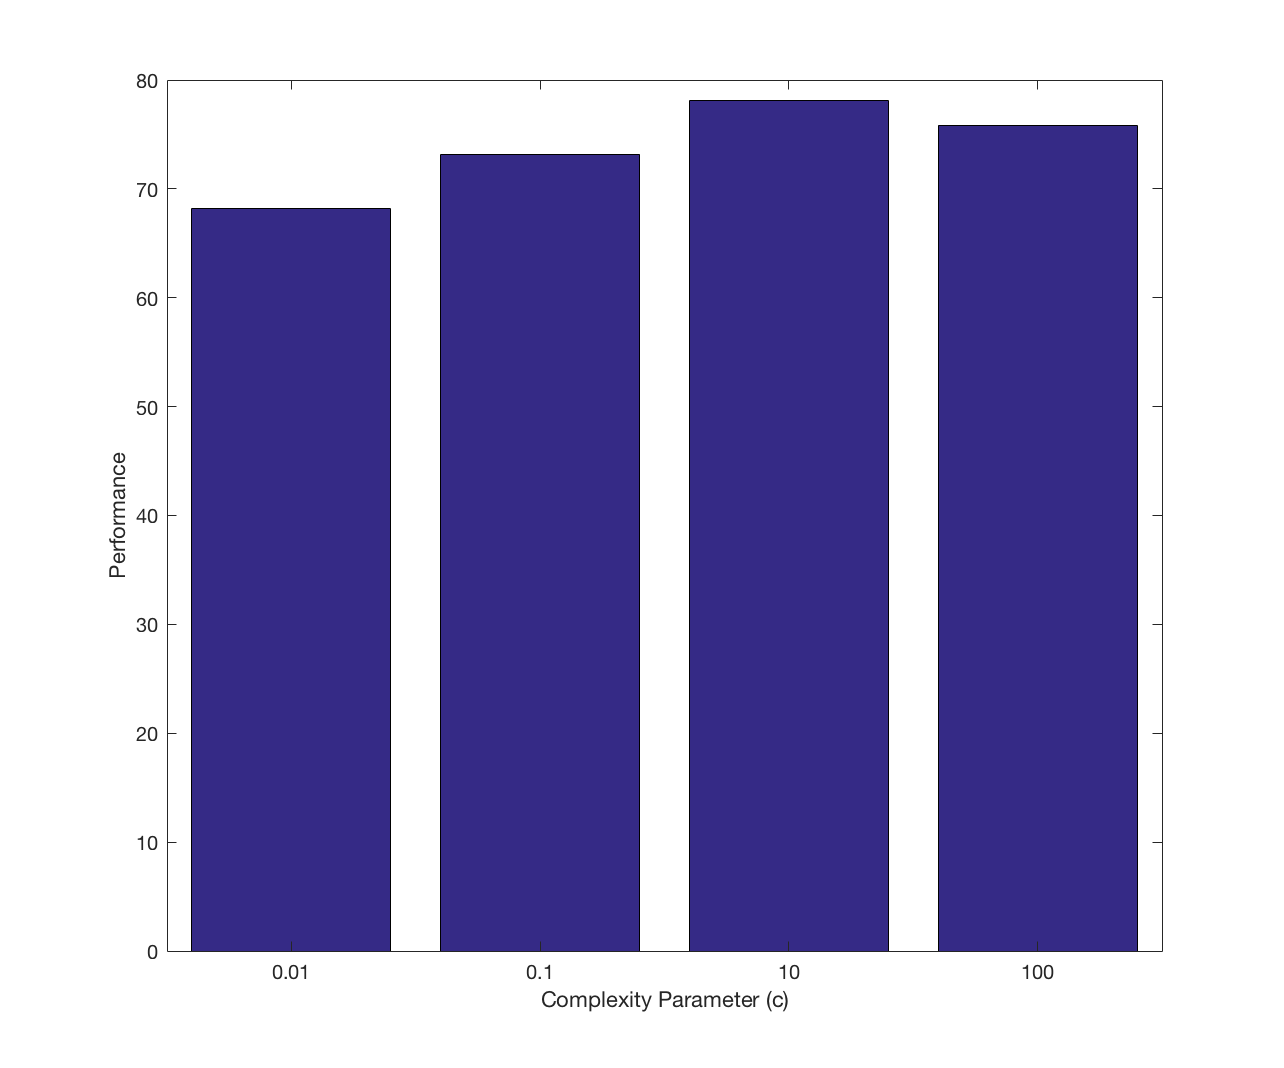
\includegraphics[width=0.7\linewidth]{../../pracs/prac8/q3}
\end{figure}

It can be seen from the graph that a perplexity of 10 produced the best performance for the given dataset.

\section*{Prac 9}

\subsection*{Q 9.5}

The methodology was adapted from the paper, the parameters are specified below
\begin{itemize}
	\item Results averaged over five standard 10 fold cross validation experiments
	\item Each dataset was partitioned into 10 equal sized datasets
	\item Each dataset is used as a test set while the classifier is trained on the other nine
	\item Each fold has an ensemble of 25 classifiers
	\item Neural networks trained with standard backpropagation
	\item Neural networks trained with a learning rate of 0.15, momentum term of 0.9, random weights between -0.5 and 0.5
\end{itemize}

\begin{table}[H]
\centering
\caption{Test Error Rates}
\begin{tabular}{|c|c|}
\hline
Data Set & Single MLP \\
\hline
diabetes & 26.3 \\
glass & 32.71 \\
ionosphere & 8.54 \\
sonar & 16.82 \\
\hline
\end{tabular}
\end{table}

The results from the table are quite similar to the paper, with the glass result having slightly smaller error than the paper.
The diabetes and sonar results are slightly higher than what was expected from the paper.

\begin{figure}[H]
	\centering
	\caption{Number of  Attributes vs Instances vs Error}
	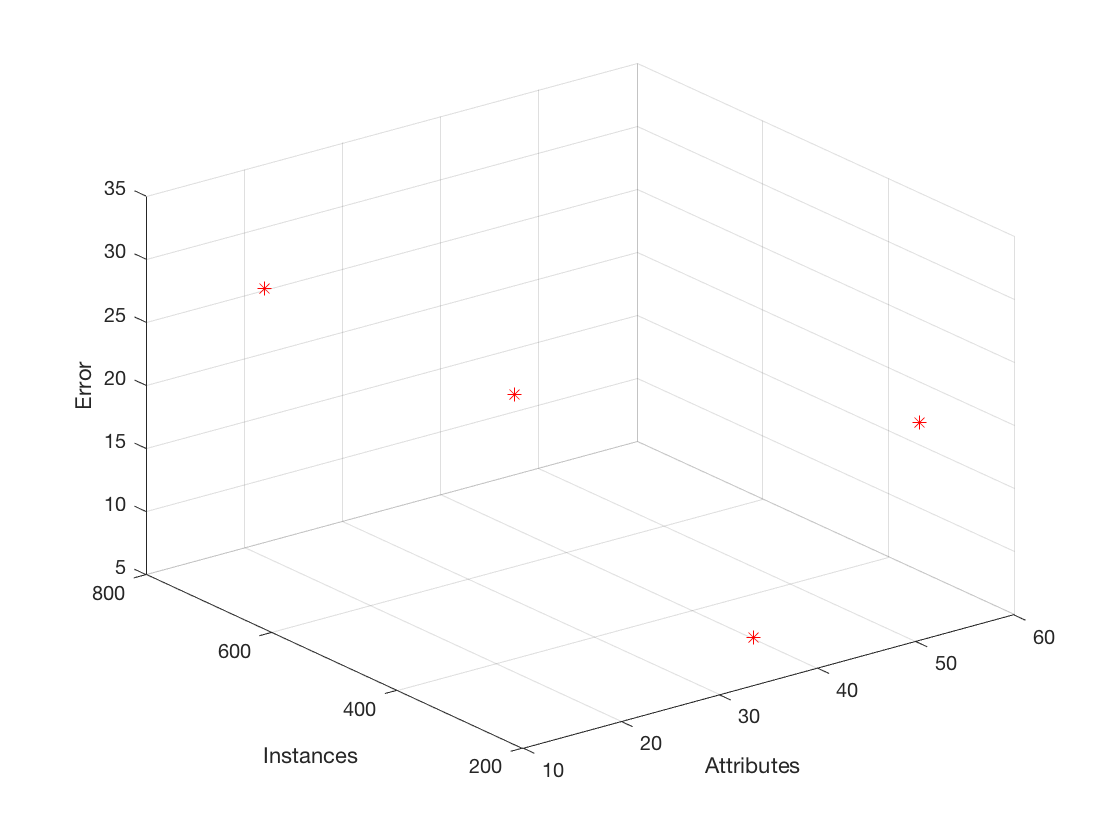
\includegraphics[width=\linewidth]{images/q9_5}
\end{figure}

The above graph is a plot of the error on the number of instances and the number of attributes.
From the graph it can be seen that there is no easily seen relationship between the data.

\subsection*{Q 9.6}

Each test was ran 5 times with different seeds and the average error was calculated, producing the following table.

Table 1 of the paper details the parameters that should be used for the neural network,
these parameters were put into Weka to generate the model.

\begin{table}[H]
\centering
\caption{Test Error Rates}
\begin{tabular}{|c|c|c|c|}
\hline
Data Set & Single MLP & Bagging & AdaBoostM1 \\
\hline
diabetes & 26.3 & 23.17 & 26.56 \\
glass & 32.71 & 31.30 & 30.84 \\
ionosphere & 8.54 & 9.11 & 8.54 \\
sonar & 16.82 & 15.38 & 16.82 \\
\hline
\end{tabular}
\end{table}

The results from the experiments are similar to the record results in the paper, with most tests being around 2\% off.
There was a few exceptions, such as the AdaBoosting for Diabetes and Sonar dataset,
which has higher error rates than what was expected from the paper.
For instance AdaBoost on the Diabetes dataset has comparable errors to a single MLP, this also occurs in the paper.
A possible reason for this is the number of instances in each dataset, as Diabetes is one of the larger datasets
with 768 instances.
Most of the other datasets that were tested had 150 to 300 entries.

The results of the paper match the experiment, with the bagging method is almost always more accurate than a single MLP.
Additionally using AdaBoost produced models which are no more accurate than a single MLP, which also matched the paper.
More specifically the paper mentioned that boosting performance can sometimes be worse when using neural networks.

The paper mentions that the performance of boosting is dependant on the data set used.
Datasets with noisy data is more likely to be overfit by boosting.

\end{document}
